\section{Future products}

\begin{itemize}
\item Noninvasive prenatal testing using circulating DNA and RNA 
\citep{moufarrej2023noninvasive}.
\item Pharmacogenomics drug dosages.
\item Pharmacogenomics drug interactions.
\item Pharmacogenomics cost effectiveness.
\item DeepInfeR
\end{itemize}


\subsection{Pharmacogenomics at Kispi}

Pharmacogenomics has the power to find direct effects of personal genetics on the metabolism and effectiveness of drugs used in the clinic. 
\textbf{Figure
\ref{fig:pharmacogenomic}}
illustrates an example of variant effect from gene-to-protein and how some gene-drug interactions are identified. 
Our pharmacogenomics strategy has a tripartite approach which is designed to personalise and enhance treatment efficacy while managing healthcare expenditures effectively.
\citet{pirmohamed2023pharmacogenomics} has reviewed the current status and future perspectives of such approaches.

Firstly, the pharmacogenomics of drug dosages focuses on adjusting medication based on genetic profiles to optimise therapeutic effects and minimise adverse reactions 
\citep{yip2015pharmacogenetic}.
By analysing a patient's genetic markers, the \pmu can predict metabolic rates and drug absorption, ensuring that each child receives a dosage that maximises benefit while reducing the risk of toxicity. 
This tailored approach not only promises better health outcomes but also reduces the trial and error typically associated with standard dosing practices.

Secondly, understanding pharmacogenomic drug interactions is crucial in a paediatric setting where polypharmacy can be common, especially in complex cases such as cancer or chronic diseases. 
The \pmu leverages genetic insights to foresee and mitigate adverse drug-drug interactions. 
This is achieved by mapping genetic variants that affect drug metabolism enzymes, transporters, and receptors, thereby providing a clear picture of potential interactions before they can cause harm.

Lastly, the aspect of cost-effectiveness in pharmacogenomics cannot be overstated. By integrating pharmacogenomic data into clinical decision-making, the \pmu aims to reduce not only the financial burden associated with ineffective treatment but also the costs related to adverse drug reactions. 
This strategic incorporation of pharmacogenomics is expected to lead to more efficient use of healthcare resources, shorter hospital stays, and fewer unnecessary tests and procedures \citep{relling2015pharmacogenomics}.

The \href{https://en.wikipedia.org/wiki/Cytochrome_P450}{Cytochrome P450} (CYP) enzymes are an especially useful target of pharmacogenomics.
These are crucial for the metabolism of many xenobiotics and endogenous compounds, making them key players in drug metabolism. 
Variations in the 15 encoding genes significantly influence drug interactions and efficacy. 
The \href{https://www.pharmvar.org}{Pharmacogene Variation} (PharmVar) consortium maintains a repository that catalogues these genetic variations, aiming to standardize nomenclature across the pharmacogenetics community
\citep{gaedigk2021pharmvar}. 
This facilitates understanding and predicting drug metabolism, disposition, and response. 
Other essential resources in this field include the 
\href{https://www.pharmgkb.org/}{Pharmacogenomic KnowledgeBase}, 
\href{https://go.drugbank.com}{DrugBank}, and 
the \href{https://cpicpgx.org/}{Clinical Pharmacogenetic Implementation Consortium}, which further support pharmacogenomic research and clinical implementation.

Over the last six years (2019-2024), our methods have been used for teaching in the EPFL master's degree coursework and hands-on projects in 
\href{https://edu.epfl.ch/coursebook/en/new-tools-research-strategies-in-personalized-health-BIO-491?cb_cycle=bama_cyclemaster&cb_section=sv}{BIO491} - MSc New tools \& research strategies in personalized health and 
\href{https://lawlessgenomics.com/topic/pharmacogenomics}{tutorials}.

\begin{figure}[h] \hspace*{-5cm} 
\begin{center}
	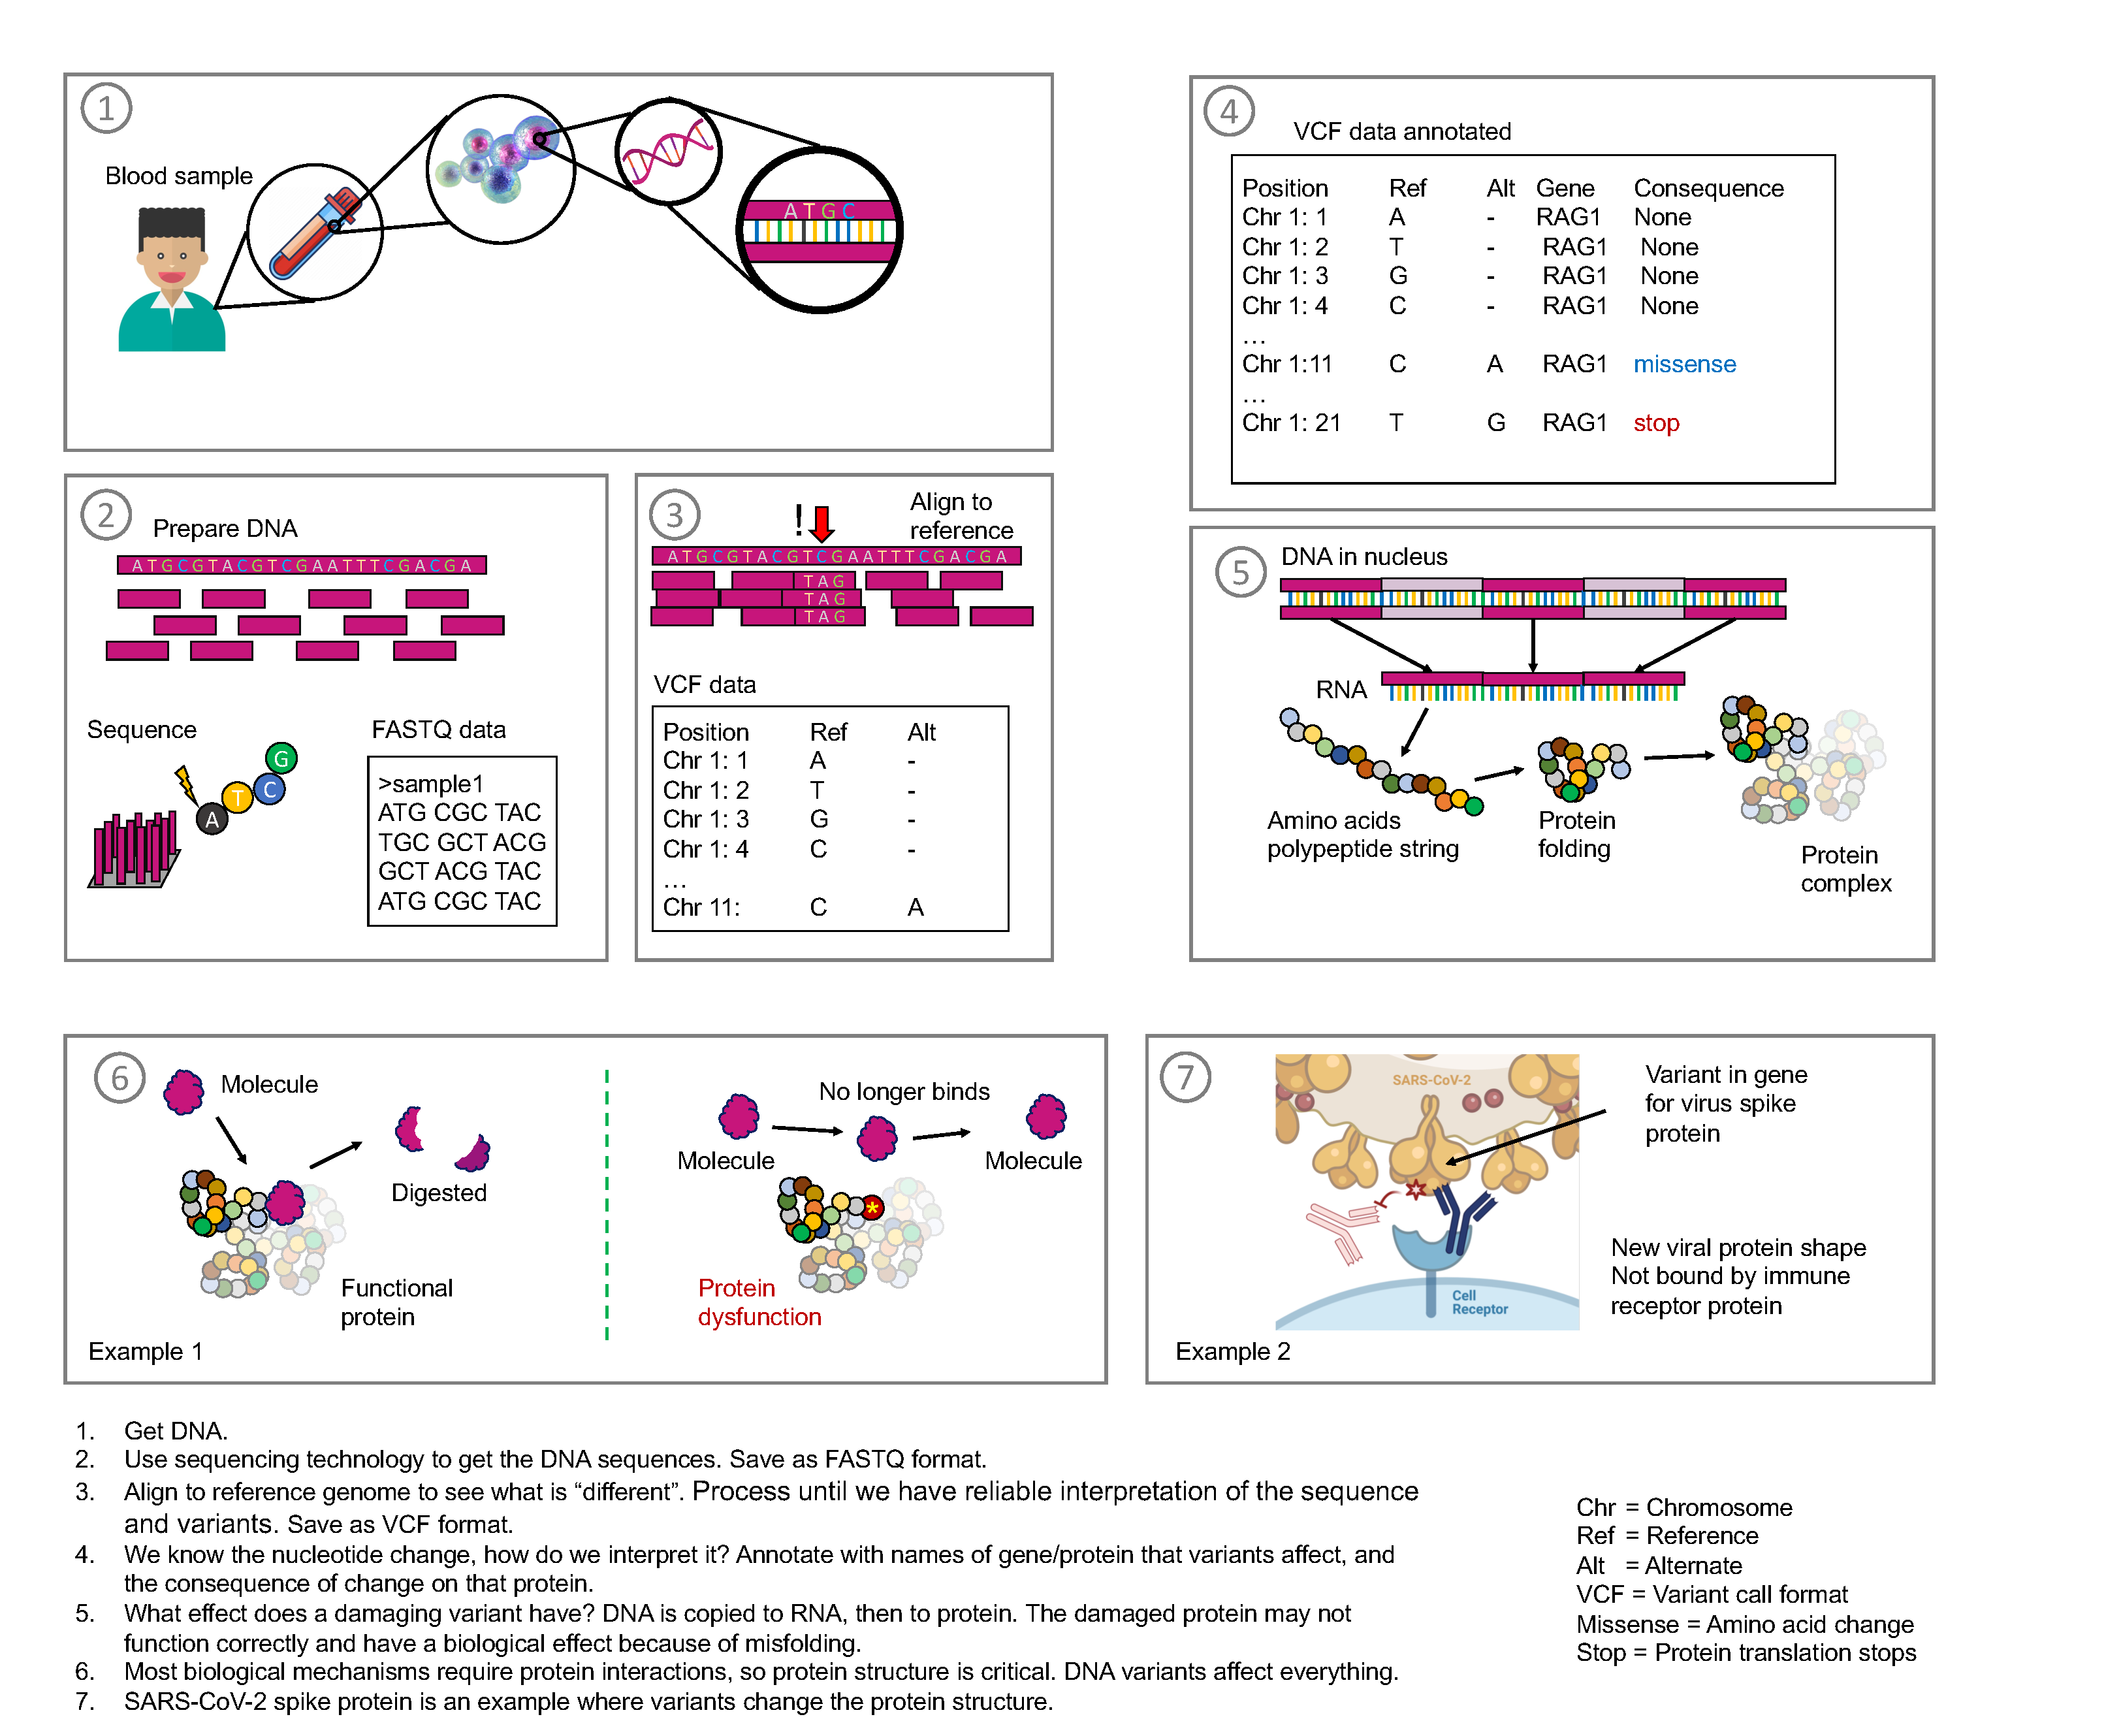
\includegraphics[width=0.55\textwidth]{DNA_to_effect}
	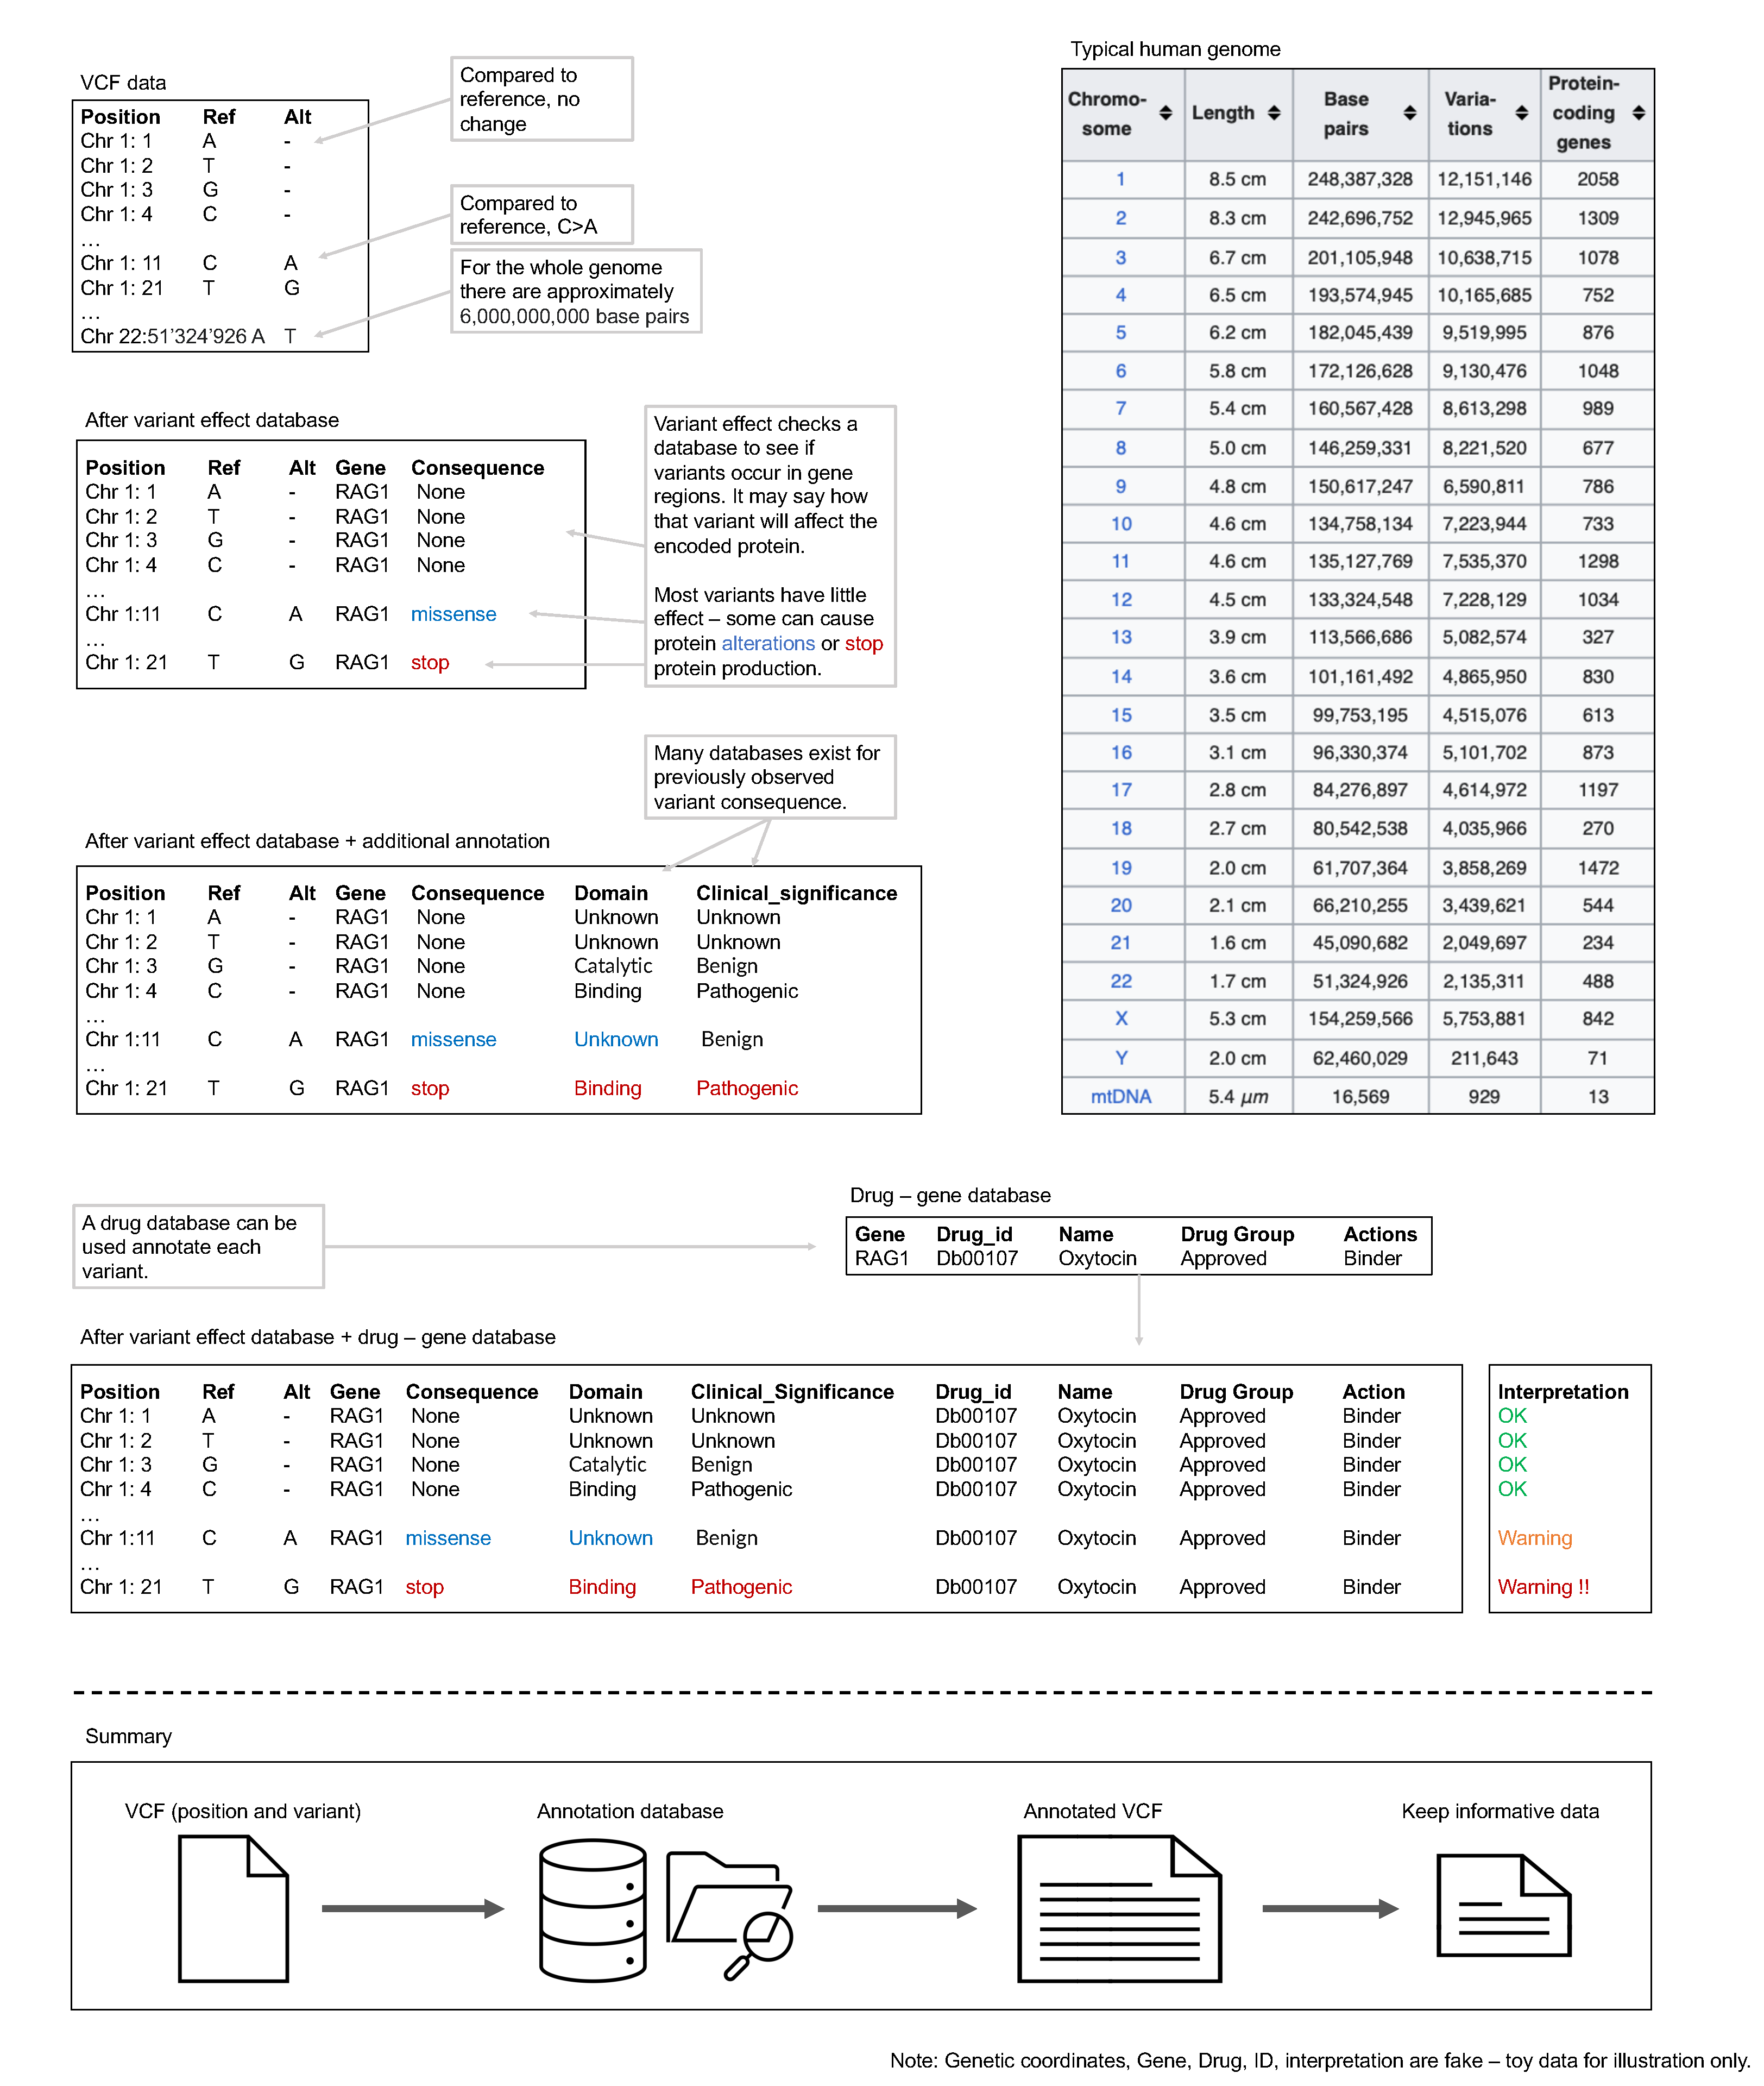
\includegraphics[width=0.40\textwidth]{effect_to_drug}
	\caption{\pmu pharmacogenomics. Known genetic variants produce measurable effects on protein and function. By applying the pharmacogeomic knowledge base to patient's personal genomic data, we can determine the gene-drug effect. This allows us to provide information about drug metabolism, dosage, indication, and cost effectiveness.}
	\label{fig:pharmacogenomic}
\end{center}
\end{figure}


\subsection{DeepInfeR}

A significant development within the \pmu is the \deepinfer initiative, which embodies our forward-thinking approach in genetic research. This project aims to pre-calculate the probability of each genetic variant, whether known or novel, in causing any given set of diseases using a comprehensive Bayesian framework. This initiative sets a new benchmark in predictive medicine by integrating extensive prior knowledge and observational data into a cohesive statistical model.

The methodology behind \deepinfer involves several rigorous steps:
\begin{enumerate}
    \item \textbf{Variant Data Collection and Annotation:} All known nucleotide variants are collected and annotated using tools such as VariantAnnotation. This annotation details the functional consequences of each variant, providing a foundational dataset for subsequent analyses.
    \item \textbf{Probability Estimation:} We estimate the frequency of each variant using population data from databases like gnomAD. Additionally, we calculate probabilities for random, novel variants that may not yet be catalogued.
    \item \textbf{Incorporation of Prior Information:} The model integrates biological data (e.g., clinical pathogenicity from ClinVar and structural data from UniProt) as Bayesian priors. This step enhances the model's ability to provide accurate estimates by including comprehensive background information.
    \item \textbf{Bayesian Inference:} Our approach updates the probability of each variant causing specific diseases by applying Bayesian inference techniques. We use statistical packages such as brms and rstan for this purpose, employing Bayes' theorem to combine prior knowledge with the observed data, resulting in a detailed set of posterior probabilities.
\end{enumerate}

This quantitative expression of disease association likelihood for each variant allows for preemptive strategies in pediatric care tailored to the genetic profiles of individual patients, significantly transforming the landscape of pediatric healthcare. The \deepinfer initiative not only broadens our understanding of genetic influences on disease but also markedly enhances our capacity to intervene effectively before clinical manifestations occur.

By continuing to refine and expand the \deepinfer initiative, we anticipate it will become a cornerstone in our predictive capabilities, providing new insights into the genetic basis of diseases and enhancing our ability to offer personalized care.
